\documentclass[conference]{IEEEtran}
\usepackage[german]{babel}
\usepackage{csquotes}
\IEEEoverridecommandlockouts
\usepackage[style=ieee]{biblatex}
\usepackage{amsmath,amssymb,amsfonts}
\usepackage{pgfplots}
\pgfplotsset{compat=1.18}
\usepackage{graphicx}
\usepackage{tabularx}
\usepackage{esvect}
\usepackage{enumitem}

\addbibresource{ROB_Projekt.bib}

\begin{document}

\title{Haptisches Feedback eines Roboters durch virtuelle 3D-Modelle}

\author{
    \IEEEauthorblockN{Carl Gathmann}
    \IEEEauthorblockA{\textit{Universität zu Lübeck} \\
        Lübeck, Germany \\
        carl.gathmann@student.uni-luebeck.de}
    \and
    \IEEEauthorblockN{Marten Buchmann}
    \IEEEauthorblockA{\textit{Universität zu Lübeck} \\
        Lübeck, Germany \\
        marten.buchmann@student.uni-luebeck.de}
}
\maketitle

\begin{abstract}
In dieser Studie wird ein Ansatz zur Erzeugung von haptischem Feedback im Bereich der Mensch-Roboter-Interaktion vorgestellt. Mittels Software wird eine haptische Wahrnehmung simuliert, die durch frei gestaltbare virtuelle 3D-Modelle gesteuert wird. Der Benutzer erfährt eine Art abstoßende Kraft, die durch die räumlichen Grenzen des virtuellen Modells definiert wird. Dadurch ist es möglich, eine physische Interaktion mit dem immateriellen Modell zu simulieren. Die vorgestellte Technologie hat viele Anwendungsbereiche, von der medizinischen Simulation über die Erkundung von Gefahrenzonen bis hin zur Steigerung des Spielerlebnisses in virtuellen Umgebungen.  

\end{abstract}

\begin{IEEEkeywords}
    Robotik, Haptisches Feedback, Mensch-Roboter-Interaktion
\end{IEEEkeywords}

\section{Einleitung}

In den vergangenen Jahren hat die Mensch-Roboter-Interaktion signifikant an Bedeutung gewonnen und sich als ein dynamisches Forschungsfeld etabliert. Im Zentrum dieses Forschungsbereichs steht die Optimierung der Benutzererfahrung, insbesondere durch die Erweiterung der menschlichen Sinneswahrnehmung.

Diese Studie präsentiert einen neuartigen Ansatz, der es Benutzern ermöglicht, mit virtuellen 3D-Modellen über ein spezialisiertes Roboterinterface in einer "fühlbaren" Weise zu interagieren. Hierzu wird eine abstoßende Kraft generiert, die auf den geometrischen Eigenschaften der virtuellen Modelle beruht. Dieses haptische Feedback dient als Simulation und ermöglicht die Annäherung an die physische Interaktion mit realen Objekten.

Das vorgestellte Verfahren hat eine Vielzahl an Anwendungen, einschließlich, aber nicht beschränkt auf, chirurgische Trainingssimulationen, die Erkundung von Umgebungen, die für den Menschen gefährlich oder unzugänglich sind, und die Intensivierung der Immersion in Virtual-Reality-Spielen. Die hier vorgestellten Methoden und technischen Implementierungen dienen als robuste Grundlage für weitere Forschungen und Entwicklungen in diesem aufstrebenden Bereich.

Der Artikel beleuchtet ausführlich die zugrunde liegenden Prinzipien, technischen Implementierungen und potenziellen Einsatzmöglichkeiten dieses Ansatzes. Dabei wird auch auf die Limitationen eingegangen, um ein umfassendes Verständnis des vorgestellten Systems zu bieten.

\section{Methoden}
Die Erzeugung des haptischen Feedbacks basiert auf der Berechnung einer abstoßenden Kraft, die so ausgelegt ist, dass sie dem Benutzer einen realistischen Eindruck von der Form des virtuellen 3D-Modells vermittelt. Die Modelle können als Datei im STL-Standard übergeben werden. Der STL-Standard speichert 3D-Modelle als Dreiecksnetz, das aus Eckpunkten und den Normalenvektoren der Dreiecke besteht. Das Format ist weit verbreitet und wird in der Industrie zum Speichern und Übertragen von 3D-Modellen verwendet. Dies gewährleistet eine hohe Flexibilität und einfache Handhabung \autocite{WasIstSTLDatei2017}.

Als Roboterarm wurde der Panda-Roboter von Franka Emika gewählt. Der Panda verfügt über 7 DOF und Kraftsensoren in allen sieben Achsen. Dadurch bietet der Manipulator eine hohe Präzision und Flexibilität, aber auch einen gewissen Sicherheitsstandard \cite{pandaDatasheet}. Ein benutzerfreundliches, 3D-gedrucktes Interface (siehe Abbildung \ref{fig:MRinterface}) ist am Endeffektor des Roboters angebracht, um die Führung durch menschliche Benutzer zu erleichtern.

\begin{figure}
    \centering
    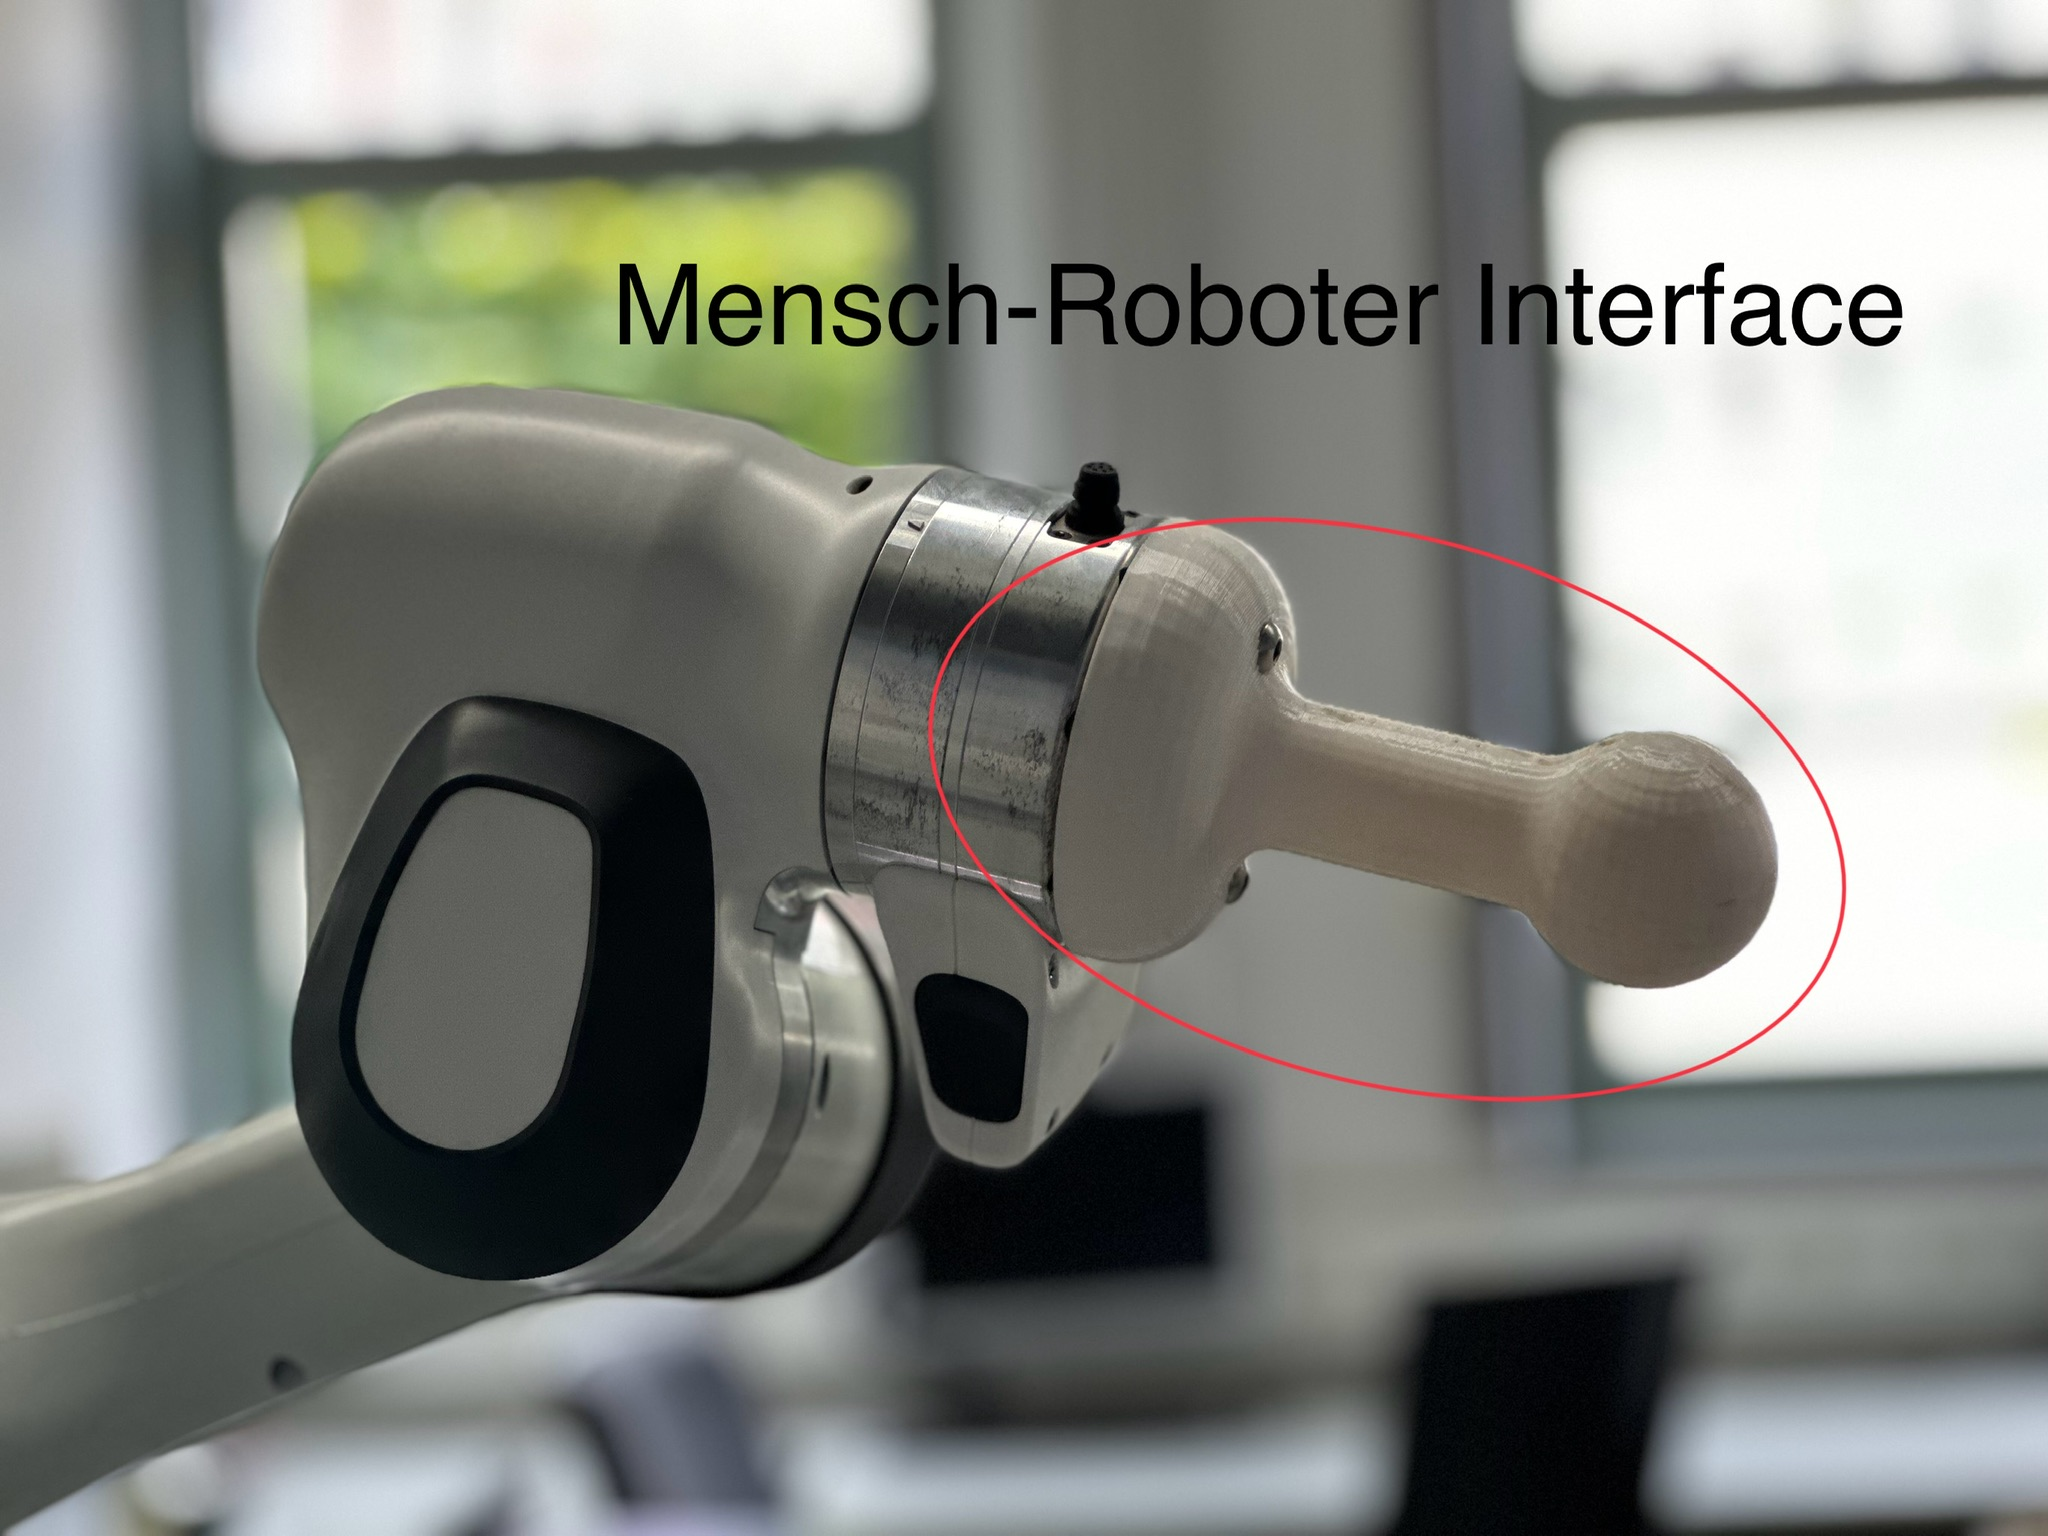
\includegraphics[width=0.45\textwidth]{pics/interface.jpeg}
    \caption{Mensch-Roboter-Schnittstelle}
    \label{fig:MRinterface}
\end{figure}

Bei der Software, die für dieses System entwickelt wird, ist die Leistung äußerst kritisch, um eine reibungslose Benutzererfahrung zu gewährleisten. Es ist von entscheidender Bedeutung, dass die Anwendung in Echtzeit mit einer maximalen Verzögerung von weniger als 1 Millisekunde ausgeführt werden kann. Die Programmiersprache C++ ist aufgrund ihrer hohen Leistungsfähigkeit geeignet, diese Anforderung zu erfüllen. Die Hardwarekonfiguration für die Umsetzung der hier vorgestellten Ergebnisse besteht aus einem Intel Core i7-3770 und 16GB RAM. Ein STL-Parser extrahiert die Eckpunkte der einzelnen Dreiecke aus der STL-Datei und speichert diese in Matrizen. Um eine einfache und effiziente Handhabung der 3D-Daten innerhalb des Programms zu ermöglichen, werden Datentypen und Funktionen aus der "Eigen"-Bibliothek verwendet. 

Im folgenden Teil werden verschiedene Ansätze vorgestellt, um aus einem Dreiecksnetz ein stetiges und kontinuierliches Vektorfeld zu erzeugen. 

\subsection*{Vorbereitung}
Als Vorbereitung auf die ersten beiden Ansätze muss zunächst das zweidimensionale Problem auf ein dreidimensionales reduziert werden. Dies wird erreicht, indem für jedes Dreieck ein neues Koordinatensystem erzeugt wird:
\begin{enumerate}
    \item Eine Kante des Dreiecks als x-Achse.
    \item Das Kreuzprodukt der resultierenden Achse mit einem anderen Vektor als z-Achse.
    \item Das Kreuzprodukt der beiden resultierenden Achsen als y-Achse.
\end{enumerate}
Die Koordinaten des Punktes werden in diesem Koordinatensystem angegeben. Auf diese Weise stellen die x- und y-Koordinaten die Position und die z-Koordinate den Abstand des Punktes von der Dreiecksebene dar.

\subsection{Kantenfunktion}\label{edge}
Die Kantenfunktion ist eine in der Computergrafik häufig verwendete Funktion. Sie wird verwendet, um die Lage eines Punktes relativ zu einer Kante \autocite{pinedaParallelAlgorithmPolygon1988} zu bestimmen. Sie ist wie folgt definiert:
\begin{equation}
    E_{i} = (x_{i+1} - x_{i})(y - y_{i}) - (y_{i+1} - y_{i})(x - x_{i})
\end{equation}
x, y sind die Koordinaten des Punktes, $x_{i}$, $y_{i}$ sind die Koordinaten des i-ten Eckpunktes des Dreiecks. Im Falle eines Dreiecks mit den Eckpunkten $A$, $B$ und $C$ und einem Punkt $P$ ist der Punkt innerhalb des Dreiecks, wenn gilt:
\begin{equation}
    E_{AB} \geq 0 \land E_{BC} \geq 0 \land E_{CA} \geq 0
\end{equation}

Mit dem Wissen, ob ein Punkt innerhalb des Dreiecks liegt und der Höhe des Punktes, die durch die z-Koordinate des transformierten Punktes gegeben ist, kann ein Kraftvektor berechnet werden. Dieser Kraftvektor zeigt in Richtung der Normalen des Dreiecks und ist proportional zur Höhe des Punktes. Die entsprechende Formel lautet:
\begin{equation}
    F = \frac{1}{z} \cdot n
\end{equation}
Dabei ist $z$ die z-Koordinate des Punktes innerhalb des Dreiecks und $n$ die Normale des Dreiecks.

\subsection{Baryzentrische Koordinaten} \label{bary}
Eine weitere Methode ist die Verwendung baryzentrischer Koordinaten. Diese Methode ist der Kantenfunktion sehr ähnlich, da sie ebenfalls verwendet wird, um die Lage eines Punktes relativ zu einem Dreieck zu bestimmen. Ein wichtiger Unterschied ist jedoch, dass auch die relative Position innerhalb des Dreiecks bestimmt werden kann. Die Koordinaten werden wie folgt berechnet:
\begin{equation*}
    \lambda_b = \pm\frac{|\Lambda(\triangle(A,P,C))|}{|\Lambda(\triangle(A,B,C))|}
\end{equation*}
\begin{equation}
    \lambda_c = \pm\frac{|\Lambda(\triangle(A,B,P))|}{|\Lambda(\triangle(A,B,C))|}
\end{equation}
\begin{equation*}
    \lambda_a = 1 - \lambda_b - \lambda_c
\end{equation*}
Dabei sind A, B, C die Eckpunkte des Dreiecks und P die in das Koordinatensystem des Dreiecks transformierte Position des Roboters. $\Lambda$ ist eine Funktion für den Flächeninhalt eines Dreiecks. $\lambda_a$, $\lambda_b$ und $\lambda_c$ sind die baryzentrischen Koordinaten des Punktes P, die angeben, wie weit der Punkt von den jeweiligen Eckpunkten entfernt ist. Sind alle drei Koordinaten positiv, so liegt der Punkt innerhalb des Dreiecks. Nun kann ein Schwellenwert festgelegt werden, ab dem zwischen den Kanten/Eckpunkten des Dreiecks interpoliert wird. Dazu muss für jede Kante bekannt sein, welche Dreiecke sie enthält und welche Normalen diese Dreiecke haben. Dasselbe gilt für die Eckpunkte. Dann kann die Kraft wie folgt berechnet werden:
\begin{equation*}
    F_{BC} = 
    \begin{cases} 
        \frac{\lambda_a}{S}\cdot N_{\triangle} + (1-\frac{\lambda_a}{S})\cdot N_{BC} &  0 < \lambda_a < \text{S} \\
        0 & \text{sonst.}
    \end{cases}
\end{equation*}
\begin{equation}
    F_{AC} = 
    \begin{cases} 
        \frac{\lambda_b}{S}\cdot N_{\triangle} + (1-\frac{\lambda_a}{S})\cdot N_{AC} &  0 < \lambda_b < \text{S} \\
        0 & \text{sonst.}
    \end{cases}
\end{equation}
\begin{equation*}
    F_{AB} = 
    \begin{cases} 
        \frac{\lambda_c}{S}\cdot N_{\triangle} + (1-\frac{\lambda_a}{S})\cdot N_{AB} &  0 < \lambda_c < \text{S} \\
        0 & \text{sonst.}
    \end{cases}
\end{equation*}
Dabei ist $N_{\triangle}$ die Normale des betrachteten Dreiecks und $N_{XY}$ die Normalen der Dreiecke, die die jeweilige Kante XY enthalten. $S$ ist ein benutzerdefinierter Schwellwert, ab dem interpoliert wird. Die resultierende Kraft $F_{XY}$ ist die Kraft, die auf den Benutzer wirkt, wenn er sich auf der Kante zwischen den Punkten X und Y bewegt.

Ein ähnlicher Ansatz gilt für die Eckpunkte. Dementsprechend wird die Kraft wie folgt berechnet:
\begin{equation*}
    F_{A} = 
    \begin{cases} 
        (1-\frac{\lambda_a}{S})\cdot N_{\triangle} + \frac{\lambda_a}{S}\cdot N_{A} &  S < \lambda_a < 1 \\
        0 & \text{sonst.}
    \end{cases}
\end{equation*} 
\begin{equation}
    F_{B} = 
    \begin{cases} 
        (1-\frac{\lambda_b}{S})\cdot N_{\triangle} + \frac{\lambda_b}{S}\cdot N_{B} &  S < \lambda_a < 1 \\
        0 & \text{sonst.}
    \end{cases}
\end{equation} 
\begin{equation*}
    F_{C} = 
    \begin{cases} 
        (1-\frac{\lambda_c}{S})\cdot N_{\triangle} + \frac{\lambda_c}{S}\cdot N_{C} &  S < \lambda_a < 1 \\
        0 & \text{sonst.}
    \end{cases}
\end{equation*} 

\subsection{Point-Triangle-Distance-Funktion}\label{dist}
Die tatsächlich verwendete Methode zur Berechnung des Kraftvektors basiert auf den Ergebnissen von \Citeauthor{eberlyDistancePointTriangle} \autocite*{eberlyDistancePointTriangle}. In der Arbeit wird eine Methode zur Berechnung des Punkt-Dreieck-Abstandes vorgestellt. Die Methode liefert zwei wesentliche Werte zurück:

\begin{enumerate}
    \item 'foot': Dieser Parameter repräsentiert den entsprechenden Punkt auf dem Dreieck, der $P$ am nächsten liegt (sei es eine Kante, ein Eckpunkt oder eine Flächenposition innerhalb der Dreiecksgrenzen). Dies ist der Punkt auf dem Dreieck, der den kleinsten Abstand 'dist' zu $P$ hat.
    \item 'dist': Dieser Parameter repräsentiert den minimalen Abstand zwischen $P$ und dem aktuell betrachteten Dreieck. Der Wert entspricht der kürzesten euklidischen Distanz, die von $P$ zu 'foot' gemessen wird.
\end{enumerate}


\begin{figure}[h] 
    \centering
    \begin{tikzpicture}
        \begin{axis}[
            xmin=-2, xmax=4,
            ymin=-2, ymax=4,
            axis lines=center,
            axis on top=true,
            domain=0:1,
            ylabel=$t$,
            xlabel=$s$,
            xtick=false,
            ytick=false,
            ]
            \addplot [dashed, line width = 1pt] coordinates {(-1,3) (3,-1)};
            \addplot [dashed, line width = 1pt] coordinates {(-1,0) (3.5,0)};
            \addplot [dashed, line width = 1pt] coordinates {(0,-1) (0,3.5)};

            \node at (axis cs:0.6,0.6) {R0};
            \node at (axis cs:1.5,1.5) {R1};
            \node at (axis cs:-0.5,3.25) {R2};
            \node at (axis cs:-0.5,1) {R3};
            \node at (axis cs:-0.5,-0.5) {R4};
            \node at (axis cs:1,-0.5) {R5};
            \node at (axis cs:3.25,-0.5) {R6};
        \end{axis}
    \end{tikzpicture}
    \caption{Die Unterteilung des Dreiecks in Regionen.}
    \label{fig:regions}
\end{figure}

Zur Berechnung der beiden Werte $dist$ und $foot$ wird zunächst die Darstellungsform des Dreiecks geändert. Die Eckpunkte eines Dreiecks werden in eine Ebenengleichung $T(s,t) = B + sE_0 + tE_1 $ überführt, wobei $(s,t) \in D = \{(s,t): s \geq 0, t \geq 0, s + t \leq 1 \}$ gelten muss. Der Abstand $Q(s,t)$ zwischen einem Punkt $P$ und dem Dreieck $T(s,t)$ kann durch den quadrierten euklidischen Abstand als elliptisches Paraboloid dargestellt werden:
\begin{equation}
    Q(s,t) = |T(s,t) - P|^2 = as^2 + 2bst + ct^2 + 2ds + 2et + f
\end{equation}
Mit $(s,t) \in D$. Die Koeffizienten $a,b,c,d,e,f$ lassen sich durch die Eckpunkte des Dreiecks und den Punkt $P$ berechnen \autocite*{eberlyDistancePointTriangle}. Somit kann der Punkt-Dreieck-Abstand durch Minimierung von $Q(s,t)$ bestimmt werden. Unter der Annahme, dass $E_0$ und $E_1$ linear unabhängig sind, kann $Q(s,t)$ nur ein globales Minimum haben. Das Minimum von $Q(s,t)$ kann durch Nullsetzen des Gradienten $\nabla Q(s,t)$ ermittelt werden. Daraus ergeben sich die Parameter $\tilde{t} = \frac{be-cd}{ac-b^2}$ und $\tilde{s} = \frac{bd-ae}{ac-b^2}$. Wenn $(\tilde{s}, \tilde{t}) \in D$ befindet sich der sogenannte Fußpunkt 'foot' des Punktes $P$ im Inneren des Dreiecks. Andernfalls ist der Fußpunkt auf den Kanten oder Eckpunkten des Dreiecks lokalisiert. Um die konkrete Lage des Fußpunktes zu bestimmen, wird das Dreieck wie in Abbildung \ref{fig:regions} in verschiedene Regionen unterteilt. Der genaue Fußpunkt wird mit Hilfe der Ebenenkurven von $Q(s,t)$ bestimmt. Eine Ebenenkurve eines elliptischen Paraboloids fällt als einfache Ellipse aus. Diese Ellipsen liegen in der $s, t$-Ebene und $Q(s, t)$ hat dort eine konstante Höhe. Dies vereinfacht die Berechnung, ob der Fußpunkt auf einer Kante oder einem Eckpunkt liegt.

Für die Regionen R1, R3 und R5 wird die Ebenenkurve gewählt, welche die entsprechende Kante des Dreiecks tangential berührt. Das Minimum der Funktion $Q(s,t)$ ergibt sich somit in R1 durch $Q(s,t)$, in R3 durch $Q(0,t)$ und in R5 durch $Q(s,0)$.

Die Regionen R2, R4 und R6 stellen Sonderfälle dar, bei denen sowohl die Richtung der Dreieckskante als auch die des Gradienten berücksichtigt werden müssen. Das Vorzeichen des Skalarprodukts der beiden Richtungen wird betrachtet, um die spezifische Region des Fußpunkts zu bestimmen. Dabei gilt für R2 $(1,-1)\cdot \nabla Q(0,1)$, für R4 $(1,0)\cdot\nabla Q(0,0)$ und für R6 $(-1,0)\cdot\nabla Q(1,0)$. 

Auf diese Weise kann der Fußpunkt des Punktes $P$ auf dem Dreieck bestimmt werden. Der Abstand ergibt sich aus der Länge des Vektors $\vv{P - foot}$. Um den resultierenden Kraftvektor zu berechnen, wurde das folgende Verfahren implementiert: \\
\linebreak
\textbf{Für jedes Dreieck der STL Datei:}
\begin{enumerate}
    \item Berechnung von $dist$ und $foot$ mithilfe der Point-Triangle-Distance-Funktion.
    \item Berechnung des Vektors $v$ zwischen $foot$ und der Roboterposition $P$.
    \item Wenn das Skalarprodukt von $v$ und der Normalen des Dreiecks positiv ist, wird die resultierende Kraft $F$ wie folgt ergänzt:
    \begin{equation}
        F \mathrel{\raisebox{0.19ex}{$\scriptstyle+$}}= v \cdot influence(dist)
    \end{equation}
\end{enumerate}

\begin{figure}[h]
    \centering
    \begin{tikzpicture}
        \begin{axis}[
            xmin=-0.05, xmax=0.1,
            ymin=-0.2, ymax=1.2,
            axis lines=center,
            axis on top=true,
            domain=0:1,
            ylabel=$influence$,
            xlabel=$distance$,
            xticklabels=false,
            every axis x label/.style={
                at={(ticklabel* cs:1.05)},
                anchor=west,
            },
            ]
            \addplot [dashed, line width = 1.5pt] coordinates {(-0.04,1) (-0.02,1)};
            \addplot [line width=1pt] coordinates {(-0.02,1) (0.02,1)};
            \addplot [line width=1pt] coordinates {(0.02,1) (0.05,0)};
            \addplot [line width=1pt] coordinates {(0.05,0) (0.07,0)};
            \addplot [dashed, line width = 1.5pt] coordinates {(0.07,0) (0.09,0)};

            \addplot [dashed] coordinates {(0.02,1) (0.02,0)};

            \node[label={270:0.02},inner sep=1.5pt] at (axis cs:0.02,0) {};
            \node[label={0:{$A$}},circle,fill,inner sep=1.5pt] at (axis cs:0.02,1) {};
            \node[label={45:{$B$}},label={270:0.05},circle,fill,inner sep=1.5pt] at (axis cs:0.05,0) {};
            
        \end{axis}
    \end{tikzpicture}
    \caption{Einfluss von Distanz auf resultierenden Kraftvektor $F$.}
    \label{fig:influence}
\end{figure}

Die Funktion $influence(dist)$ repräsentiert eine linear fallende Funktion innerhalb eines spezifischen Intervalls, das von 1 auf 0 abfällt (siehe Abbildung \ref{fig:influence}). Damit können die verschiedenen Einflüsse der Kraftvektoren auf den resultierenden Gesamtkraftvektor variiert werden. Ein größeres Intervall führt zu einer weicheren und runderen Haptik des simulierten Objekts. In der vorliegenden Implementierung wurde ein Intervall zwischen 5 cm und 2 cm als Parameter ausgewählt. Vektoren, die vom Punkt des minimalen Abstands zur Roboterposition ausgehen und eine Länge von weniger als 2 cm haben, gehen mit voller Intensität in die Berechnung ein. Vektoren mit einer Länge von 5 cm oder mehr werden von der Berechnung ausgeschlossen. Für alle dazwischen liegenden Vektorlängen wird eine lineare Interpolation durchgeführt.

Zur Visualisierung der Kräfte für verschiedene Punkte wurde ein Vektorfeld erstellt (siehe Abbildung \ref{fig:vectorfield}). Man kann klar erkennen, dass keine Unstetigkeiten entlang der Kanten und Eckpunkte auftreten.
\begin{figure}[h]
    \centering
    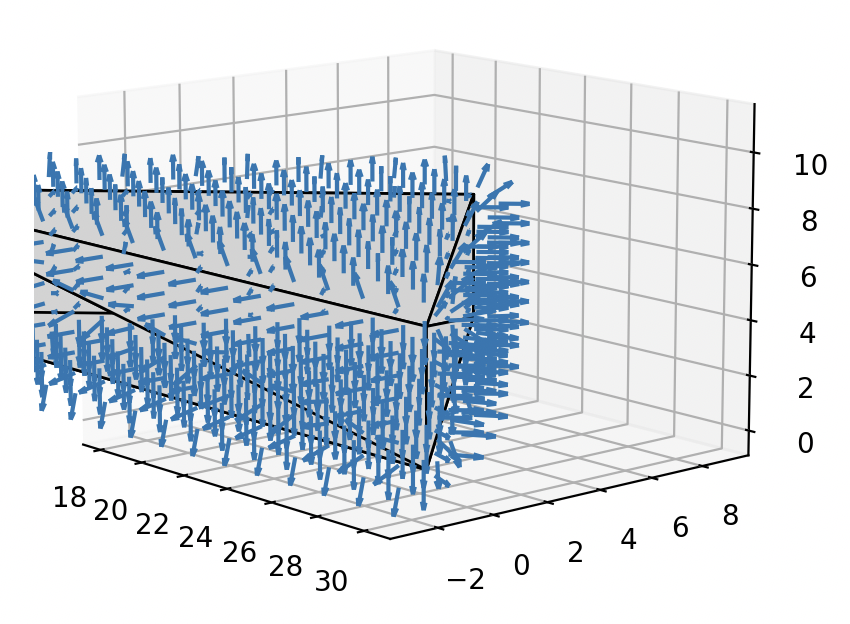
\includegraphics[width=0.5\textwidth]{pics/vectorfield.png}
    \caption{Vektorfeld Visualisierung.}
    \label{fig:vectorfield}
\end{figure}
\section{Ergebnisse}
\subsection{Effekt}

Bei der Überprüfung der Implementierung konnte festgestellt werden, dass der beabsichtigte Effekt der abstoßenden Kraft sowie der gewünschte Eindruck von Plastizität erfolgreich erzielt wurden. Die Kanten und Ecken der in der STL-Datei definierten Struktur waren deutlich zu erkennen. Ein kurzes Demonstrationsvideo, das die Funktionsweise und das Ergebnis der angewandten Implementierung veranschaulicht, kann unter dem folgenden Link angesehen werden:
\begin{minipage}{\textwidth}
    \nobreak\url{https://youtu.be/IhARjkxuTvw}.
\end{minipage}

\subsection{Performanz}
Hinsichtlich der Leistung wurden ebenfalls zufriedenstellende Ergebnisse erzielt. Bei der Verarbeitung einer STL-Datei mit 160 Dreiecken betrug die durchschnittliche Berechnungszeit für den Kraftvektor eines Punktes auf der oben beschriebenen Hardware nur 0,714 Millisekunden. Im Kontext einer Echtzeitanwendung stellt dieser Wert einen akzeptablen Rechenaufwand dar.

\section{Diskussion}
Die Methode \ref*{edge} zeichnet sich durch ihre Einfachheit und Schnelligkeit aus. Sie bietet jedoch keine Möglichkeit, zwischen den Dreiecken zu interpolieren. Dadurch entstehen Unstetigkeiten an den Kanten der Dreiecke, was zu einem unintuitiven und sprunghaften Verhalten führt, wenn sich der Benutzer entlang der Kante bewegt.

Der Vorteil von \ref*{bary} gegenüber \ref*{edge} ist, dass Unstetigkeiten entlang von Kanten vermieden werden. Allerdings ist die Berechnung der baryzentrischen Koordinaten komplexer und langsamer. Außerdem müssen zur Interpolation der verschiedenen Dreiecksflächen die Nachbarschaftsbeziehungen bestimmt werden. Somit ist der Rechenaufwand pro Roboterposition deutlich höher.

Die Methode \ref*{dist} ist in der Lage, ein lückenloses Vektorfeld zu erzeugen und weist dennoch eine gute Performance auf. Allerdings liegt die Laufzeit bei unserer Implementierung in $O(n)$, was zu Skalierungsproblemen führt. Wenn die STL-Dateien eine bestimmte Größe überschreiten, kann die Forderung nach Echtzeitfähigkeit nicht mehr zuverlässig erfüllt werden. Mögliche Ansätze zur Verbesserung der Performance wären:
\begin{enumerate}
    \item Das Parallelisieren der Berechnungen durch das Einsetzen der GPU.
    \item Level of Detail (LOD) Modelle, wie sie in der Computergrafik verwendet werden.
    \item Nutzung von Octrees.
    \item Nutzung von leistungsstärkerer Hardware.
\end{enumerate}
Durch die Anwendung dieser Methoden könnte die Echtzeitanforderung des Systems auch bei umfangreicheren STL-Dateien erfüllt werden.

\section{Fazit}
Zusammenfassend kann gesagt werden, dass es mit \ref*{dist} gelungen ist, eine effiziente Methode zur Erzeugung eines haptischen Feedbacks zu entwickeln. Durch die Verwendung des STL-Standards können beliebige Modelle entworfen und in stetige Vektorfelder umgewandelt werden. Die vorgestellte Methode zur Erzeugung von haptischem Feedback eines Roboters durch virtuelle 3D-Modelle kann somit in verschiedenen Anwendungsbereichen eingesetzt werden.

\printbibliography

\end{document}
